\chapter{Estudi en profunditat de l'API de FamilySearch}

    \paragraph{}
    Abans de començar amb aquest apartat de la memòria, recordar que aquesta està basada en la documentació oficial de FamilySearch i complementada amb les investigacions que s'han realitzat durant el projecte.

    Com ja hem comentat, la documentació oficial està trossejada en moltes petites parts i manca d'un ordre de lectura clar que permeti comprendre l'estructura gene\-ral de l'API i les dades accessibles. De fet, quan s'accedeix a la plataforma per desenvolupadors, el primer que es veu és una llista d'operacions llarguíssima, que no serveix de gaire a una persona que es vulgui iniciar en la utilització de l'API.

    Per aquest motiu, en aquesta secció de la memòria, rescatem totes les petites peces d'informació valuoses perdudes per la documentació de FamilySearch i la presentem d'una forma que permet obtenir una idea general de l'estructura de l'arbre familiar, els principals recursos accessibles, com aquestes es troben connectats els uns amb els altres i les petites peces d'informació genealògica accessibles.

    \section{Els recursos de FamilySearch}

    \paragraph{}
    L'API de FamilySearch organitza tota la informació disponible en objectes que són anomenats recursos.

    Cada recurs emmagatzema informació relativa al concepte que representa. Per exemple, el recurs Persona conté informació sobre si aquesta està viva o morta, el seu nom i tota mena d'informació i esdeveniments relacionats amb la seva vida.

    En la taula~\ref{ref:personGedcom} de la secció anterior de la memòria, observàvem ja, com a exemple, alguns dels paràmetres continguts pel recurs Persona de l'API de FamilySearch.

    El recursos també es caracteritzen per emmagatzemar informació relativa a quines operacions es poden realitzar sobre ells. Per exemple, el recurs Persona, conté informació sobre com accedir a les operacions llegir una persona, editar una persona, esborrar una persona, buscar possibles duplicats de la persona, etcètera.

    Finalment, els recursos també destaquen per contenir els enllaços o més ben dit, les URIs, als recursos relacionats. Parlarem més en detall d’aquestes URI en el següent apartat de la memòria.

    \section{Enllaços hypermedia, la navegació entre recursos}

    \paragraph{}
    Com hem comentat en l’apartat anterior, els recursos emmagatzemen informació sobre les URI dels recursos relacionats. Aquestes URI són anomenades enllaços hypermedia i permeten la navegació  entre els diferents recursos del model de dades.

    Per posar un exemple, imaginem-nos el recurs Persona d'un individu en concret. Aquest, conté enllaços hypermedia que apunten als recursos que conformen el concepte Parella, Pares, Fills, Fonts d'informació, Ascendència, Descendència i Memòries, de la persona en concret. Com es de suposar, cada un d'aquets rescursos enllaçats, conté informació d'interès sobre la persona consultada.

    La figura~\ref{fig:hypermedia} reflecteix com el recurs Persona és accessible a través de l'Arbre Familiar de FamilySearch i com les diferents relacions i recursos associats a aquest són connectats a través dels enllaços hypermedia.

    \begin{figure}[h]
        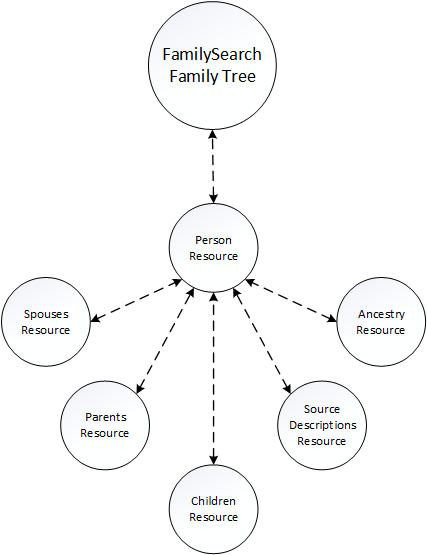
\includegraphics[scale=0.8]{05/01_hypermedia}
        \centering
        \caption{Enllaços hypermedia del recurs Persona.}\label{fig:hypermedia}
    \end{figure}

    Volem aprofitar aquest apartat de la memòria per recordar, que en el moment en què la nova versió del back-end, Family Tree, es trobi desplegada per complet a producció, el recurs Persona no contindrà més els enllaços hypermedia a tots aquests recursos, sinó que les relacions de parella o paternals, es trobaran incloses dins del mateix recurs Persona.

    De totes maneres, el concepte dels enllaços hypermedia seguirà sent vàlid de cara a les relacions del recurs Persona amb la resta de recursos vinculats i per tota la resta de relacions entre els diferents recursos de l'API de FamilySearch.

    Els enllaços hypermedia cobren especial interès a l'hora de crear aplicacions robustes que es vegin el menys afectades possible per canvis en la localització o crida dels recursos.

    El primer gran avantatge d’utilitzar aquests enllaços és que no cal implementar en el codi, de forma específica, les URI d'accés a cada recurs. D'aquesta forma, s'aconsegueix evitar que en cas de canvi en les URI dels recursos, sigui necessari realitzar modificacions en el codi de les nostres aplicacions.

    El segon avantatge, és que si es coneix un sol punt d’entrada al sistema, les aplicacions ja no requeriran més informació per tal de navegar entre els diferents recursos de l'arbre familiar. D'aquesta forma, podríem descriure els enllaços hypermedia, com una espècie d'índexs que permeten navegar i explorar el conjunt de recursos relacionats, de les respostes retornades per l'API de FamilySearch.

    \section{L'arbre genealògic de FamilySearch}

    \paragraph{}
    El model de dades que conforma l'arbre genealògic de FamilySearch, consta de molts recursos i enumeracions diferents. No citem en la memòria el nombre total de recursos diferents, ja que alguns dels objectes documentats de forma oficial es troben en desús, mentre que alguns objectes nous, encara no han rebut la documentació pertinent.

    El conjunt d'objectes o recursos connectats, conformen el que ha estat enomenat l'arbre familiar de FamilySearch (Family Tree). Aquest arbre, pot ser subdividit en cinc grans blocs:

    \begin{itemize}
        \item \textbf{El bloc de persones:} Aquest bloc representa al conjunt de recursos que emmagatzemen la informació personal de les diferents persones representades a l'arbre familiar.
        \item \textbf{El bloc de les relacions familiars:} Aquest bloc està format per aquells recursos que contenen informació sobre les diferents relacions familiars entre les persones emmagatzemades en el sistema.
        \item \textbf{El bloc de col·leccions:} Aquest bloc recull els recursos que guarden la informació relativa a les fonts de dades i documents digitalitzats, que certifiquen la veracitat de les dades.
        \item \textbf{El bloc de discussions:} El bloc de discussions conté aquells recursos que contenen la informació relativa a les converses o discussions creades, per part dels usuaris, al voltant de les persones de l'arbre familiar.
        \item \textbf{El bloc de memòries:} Aquest últim bloc està format per aquells recursos que emmagatzemen la informació relativa a les memòries descrites en la secció tres d'aquesta memòria.
    \end{itemize}

    La imatge~\ref{fig:familyTree} mostra aquests cinc grans blocs que conformen l'arbre familiar de FamilySearch i com es troben relacionats entre ells.

    \begin{figure}[h]
        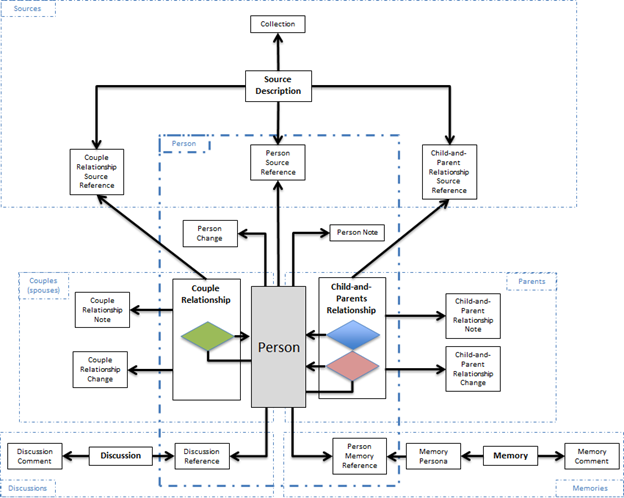
\includegraphics{05/02_overallModel}
        \centering
        \caption{Estructura de l'arbre familiar de FamilySearch}\label{fig:familyTree}
    \end{figure}

    Els blocs principals de l'arbre familiar són, sense cap mena de dubte, els que contenen la informació relativa a les persones i a les relacions familiars que les lliguen.

    L’objectiu de la resta de blocs que conformen l'arbre familiar és el de proporcionar suport i informació extra més detallada sobre les persones, relacions familiars, veracitat de les dades i investigacions realitzades sobre aquestes persones i línies genealògiques.

    En els següents apartats de la memòria s'estudiarà el conjunt de recursos principals que conformen cada bloc de l'arbre familiar i quines són les diferents peces d'informació accessibles a través de cada un d'aquests recursos.

    No es representarà en aquest projecte el conjunt total d'operacions diferents que pot ser realitzat sobre els diferents recursos, ja que les possibilitats de configuració d'aquestes són molt elevades i no té gaire sentit duplicar tota la documentació oficial respecte aquest punt.

    Tanmateix, sí que volem mencionar que gairebé tots els recursos que formen part del model de dades de FamilySearch, poden ser sotmesos als següents grups d'operacions:

    \begin{itemize}
        \item \textbf{Lectura:} Tots els recursos són, evidentment, llegibles. Cada un dels recursos conté diferents opcions de lectura i generalment, també solen ser personalitzables mitjançant la inclusió de diferents paràmetres.
        \item \textbf{Actualització:} Sempre que es disposi dels permisos adequats sobre les dades, els usuaris també poden realitzar operacions d'actualització per corregir errors, modificar la informació existent o bé afegir nova informació.
        \item \textbf{Esborrat:} Si es disposa dels permisos suficients, els usuaris poden esborrar informació incorrecta o duplicada dels diferents recursos, o el recurs sencer, mitjançant les operacions d'esborrat.
        \item \textbf{Creació:} En cas de voler afegir noves peces d'informació a les bases de dades de FamilySearch, siguin noves persones o informació específica relacionada a alguna persona que ja es troba en el sistema, això és realitzable a través de les operacions de creació de cada recurs.
    \end{itemize}

    Dit això, passem doncs a analitzar els principals recursos de cada bloc de l'arbre familiar i les peces d'informació més destacables que els conformen.

    \section{Recursos principals del bloc Persones}

    \paragraph{}
    El centre d'aquest bloc de recursos és el recurs Persona. Aquest recurs, emmagatzema els detalls que identifiquen i caracteritzen a cada una de les persones de l'arbre així com la informació bàsica sobre els seus relatius més propers.

    D'aquest recurs principal, pengen els enllaços cap als recursos que permeten obtenir informació sobre els relatius de la persona, els estudis realitzats sobre aquesta, l'historial de canvis, les fonts d'informació i les memòries afegides pels usuaris.

    La imatge [ref] ofereix una visió de l'esquema que acabem de descriure i permet veure com el recurs Persona s'enllaça amb la resta de blocs que conformen l'arbre familiar~\ref{img:personsBloc}.

    \begin{figure}[h]
        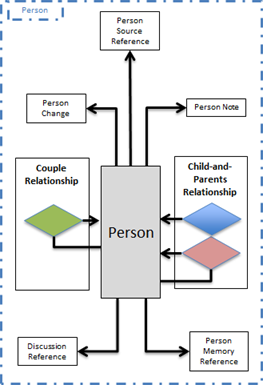
\includegraphics{05/03_personsCore}
        \centering
        \caption{El bloc de l'arbre familiar relatiu a les Persones.}\label{img:personsBloc}
    \end{figure}

    Aquest bloc de recursos és el més gran de tots i pràcticament, emmagatzema tota la informació rellevant dels individus accessibles a través de l'API. En els següents subapartats s'exposaran els diferents recursos que conformen aquest bloc i quines són les peces d'informació utilitzables que aquests contenen.

    Podreu observar, en les taules que representen l'estructura dels recursos, que a vegades, per la columna que marca el format de dades d'un paràmetre, aquest es troba especificat entre els caràcters `[' i `]'. Aquesta terminologia s'utilitza per indicar que aquest paràmetre és en realitat un recurs o objecte de dades diferent inclòs dins del recurs estudiat.

    També s'observarà que sovint, els recursos exposats, hereten dades d'altres recursos i en els casos que aquests siguin rellevants, se n'exposarà l'estructura a l'apartat `Altres recursos interessants', més endavant en la memòria.

    \subsection{El recurs Persona (Person)}

    \paragraph{}
    El recurs Persona és el primer objecte amb què cal familiaritzar-se per tal de comprendre la potencialitat emmascarada d'aquesta API.

    Cada instància, fa referència a una persona diferent de l'arbre familiar i generalment, representa el punt d'entrada per tal d'accedir a tota la informació disponible sobre un individu, ja sigui perquè aquesta es troba inclosa en el recurs o esdevé accessible a través dels enllaços hypermedia.

    Els enllaços hypermedia del recurs Persona permeten accedir a la informació relativa als seus avantpassats, descendents, artefactes, historial de canvis, parelles, discussions, notes i fonts de dades.

    Les dades pròpies pel recurs Persona poden ser observades a la taula~\ref{tab:person}. Cal recordar que aquest recurs també hereta els paràmetres dels recursos Subjecte, Conclusió, Enllaços Hypermedia i Dades Extensibles que poden ser trobats a la secció `Altres recursos interessants'.

    \begin{center}
             \csvreader[
                separator=comma,
                before table=\sffamily\small,
                longtable={p{2cm-2\tabcolsep}p{3.5cm-2\tabcolsep}p{8.5cm-2\tabcolsep}},
                table head={\caption{Codificació GEDCOM X del recurs Persona}\label{tab:person}\\\toprule%
                    \headentry{m{2cm-2\tabcolsep}}{Paràmetre}
                    & \headentry{m{3.4cm-2\tabcolsep}}{Format de Dades}
                    & \headentry{m{8.5cm-2\tabcolsep}}{Descripció}\\\midrule},
                late after line=\\\midrule,
                late after last line=\\\bottomrule,
             ]
             {./tables/05/01_persons/person.csv}
             {param=\param,format=\format,desc=\desc}
             {\param&\format&\desc}
     \end{center}

    \subsection{El recurs Gènere (Gender)}

    \paragraph{}
    El recurs Gènere s'utilitza per especificar el gènere d'una persona en concret. Aquest recurs conté els paràmetres propis mostrats a la taula~\ref{tab:gender} i hereta els camps de dades dels recursos Conclusió, Enllaços Hypermedia i Dades Extensibles que poden ser trobats a la secció `Altres recursos interessants'.

    \begin{center}
             \csvreader[
                separator=comma,
                before table=\sffamily\small,
                longtable={p{2cm-2\tabcolsep}p{3.5cm-2\tabcolsep}p{8.5cm-2\tabcolsep}},
                table head={\caption{Codificació GEDCOM X del recurs Persona}\label{tab:gender}\\\toprule%
                    \headentry{m{2cm-2\tabcolsep}}{Paràmetre}
                    & \headentry{m{3.4cm-2\tabcolsep}}{Format de Dades}
                    & \headentry{m{8.5cm-2\tabcolsep}}{Descripció}\\\midrule},
                late after line=\\\midrule,
                late after last line=\\\bottomrule,
             ]
             {./tables/05/01_persons/gender.csv}
             {param=\param,format=\format,desc=\desc}
             {\param&\format&\desc}
     \end{center}


     \subsubsection{L'enumeració genderType}

     \paragraph{}
     L'enumeració genderType segueix l'estructura de definició GEDCOMX. Com a tal, els valors possibles per l'enumeració segueixen la pauta:

     http://gedcomx.org/ + `genderType'

     La següent taula mostra els tres possibles valors de l'enumeració genderType.

     \begin{center}
         \csvreader[
            no head,
            separator=comma,
            table head={\caption{Valors possibles per l'enumeració genderType}\label{tab:genderType}},
            before table=\sffamily\small,
            longtable={|p{3cm}|p{3cm}|p{3cm}|},
            column count=4,
            late after head=\\\hline,
            late after line=\\\hline,
            late after last line=\\\hline,
         ]
         {./tables/05/01_persons/genderType.csv}
         {1=\one,2=\two,3=\three}
         {\one&\two&\three}
     \end{center}

    \subsection{Els recursos Nom, Forma del Nom i Part del Nom (Name, NameForm, NamePart)}

    \paragraph{}
    Aquest conjunt de recursos s'utilitza per representar la informació relativa als noms d'una persona.  Contenen informació sobre si un nom és el preferit de cara a ser utilitzat com a nom principal, en quin moment la persona va adoptar aquest nom i diferents formes de representació.

    Resulta útil poder accedir a diferents noms d'una mateixa persona, per poder alternar, per exemple, entre el seu mot i el nom en el moment de naixement o defunció.

    El recurs Nom està format pels paràmetres mostrats a la taula~\ref{res:name} i hereta també els paràmetres dels recursos Conclusió, Enllaços Hypermedia i Dades Extensibles que poden ser trobats a la secció `Altres recursos interessants'.

    Per altre banda, els recursos Forma del Nom i Part del Nom, contenen els paràmetres mostrats a les taules~\ref{res:nameForm} i~\ref{res:namePart} respectivament i hereten els paràmetres del recurs Dades Extensibles descrit en l'apartat `Altres recursos interessants'.

    \begin{center}
             \csvreader[
                separator=semicolon,
                before table=\sffamily\small,
                longtable={p{2cm-2\tabcolsep}p{3.5cm-2\tabcolsep}p{8.5cm-2\tabcolsep}},
                table head={\caption{Paràmetres del recurs Nom}\label{res:name}\\\toprule%
                    \headentry{m{2cm-2\tabcolsep}}{Paràmetre}
                    & \headentry{m{3.4cm-2\tabcolsep}}{Format de Dades}
                    & \headentry{m{8.5cm-2\tabcolsep}}{Descripció}\\\midrule},
                late after line=\\\midrule,
                late after last line=\\\bottomrule,
             ]
             {./tables/05/01_persons/name.csv}
             {param=\param,format=\format,desc=\desc}
             {\param&\format&\desc}
     \end{center}

     \begin{center}
         \csvreader[
         separator=comma,
         before table=\sffamily\small,
         longtable={p{2cm-2\tabcolsep}p{3.5cm-2\tabcolsep}p{8.5cm-2\tabcolsep}},
         table head={\caption{Paràmetres del recurs Forma del Nom}\label{res:nameForm}\\\toprule%
         \headentry{m{2cm-2\tabcolsep}}{Paràmetre}
         & \headentry{m{3.4cm-2\tabcolsep}}{Format de Dades}
         & \headentry{m{8.5cm-2\tabcolsep}}{Descripció}\\\midrule},
         late after line=\\\midrule,
         late after last line=\\\bottomrule,
         ]
         {./tables/05/01_persons/nameForm.csv}
         {param=\param,format=\format,desc=\desc}
         {\param&\format&\desc}
     \end{center}

     \begin{center}
         \csvreader[
         separator=semicolon,
         before table=\sffamily\small,
         longtable={p{2cm-2\tabcolsep}p{3.5cm-2\tabcolsep}p{8.5cm-2\tabcolsep}},
         table head={\caption{Paràmetres del recurs Part del Nom}\label{res:namePart}\\\toprule%
         \headentry{m{2cm-2\tabcolsep}}{Paràmetre}
         & \headentry{m{3.4cm-2\tabcolsep}}{Format de Dades}
         & \headentry{m{8.5cm-2\tabcolsep}}{Descripció}\\\midrule},
         late after line=\\\midrule,
         late after last line=\\\bottomrule,
         ]
         {./tables/05/01_persons/namePart.csv}
         {param=\param,format=\format,desc=\desc}
         {\param&\format&\desc}
     \end{center}

     \subsubsection{L'enumeració nameType}

     \paragraph{}
     L'enumeració nameType segueix l'estructura de definició GEDCOMX. Com a tal, els valors possibles per l'enumeració segueixen la pauta:

     http://gedcomx.org/ + `nameType'

     La següent taula mostra els possibles valors de l'enumeració nameType.

     \begin{center}
         \csvreader[
            no head,
            separator=comma,
            table head={\caption{Valors possibles per l'enumeració nameType}\label{enum:nameType}},
            before table=\sffamily\small,
            longtable={|p{3cm}|p{3cm}|p{3cm}|p{3cm}|},
            column count=4,
            late after head=\\\hline,
            late after line=\\\hline,
            late after last line=\\\hline,
         ]
         {./tables/05/01_persons/nameType.csv}
         {1=\one,2=\two,3=\three,4=\four}
         {\one&\two&\three&\four}
     \end{center}


   \subsubsection{L'enumeració namePartType}

   \paragraph{}
   L'enumeració namePartType segueix l'estructura de definició GEDCOMX. Com a tal, els valors possibles per l'enumeració segueixen la pauta:

   http://gedcomx.org/ + `namePartType'

   La següent taula mostra els possibles valors de l'enumeració namePartType.

   \begin{center}
       \csvreader[
          no head,
          separator=comma,
          table head={\caption{Valors possibles per l'enumeració namePartType}\label{enum:namePartType}},
          before table=\sffamily\small,
          longtable={|p{3cm}|p{3cm}|p{3cm}|p{3cm}|},
          column count=4,
          late after head=\\\hline,
          late after line=\\\hline,
          late after last line=\\\hline,
       ]
       {./tables/05/01_persons/namePartType.csv}
       {1=\one,2=\two,3=\three,4=\four}
       {\one&\two&\three&\four}
   \end{center}

   El fet que es puguin configurar valors diferents per cada part del nom i diferents noms per la mateixa persona, cobra certa importància, ja que per exemple, en els baptismes del catolicisme, es solen utilitzar tres noms de pila diferents.

   Un altre exemple, potser encara més clar, del benefici d'utilitzar aquest conjunt de recursos per definir els noms d'una persona, resideix en les diferencies d'ús dels cognoms arreu del món. Per exemple, als Estats Units, les persones només tenen un cognom, mentre que a Espanya i altres països, en tenim dos. A més a més, en molts països europeus, el cognom d'una persona canvia segons el seu estat civil (solter, casat, vidu, etcètera) i per tant, existeix un clar benefici en poder emmagatzemar-ne més d'un.

    \subsection{El recurs Esdeveniment (Fact)}

    \paragraph{}
    El recurs Esdeveniment, tal com el seu nom indica, conté informació sobre un esdeveniment relacionat a la vida d'una persona o relació familiar. En concret, proporciona detalls sobre el tipus d'esdeveniment del quel es tracta, així com la data i localització on va succeir.

    Aquest recurs està format pels paràmetres mostrats a la taula~\ref{res:fact} i els paràmetres heretats dels recursos Conclusió, Enllaços Hypermedia i Dades Extensibles que poden ser trobats a la secció `Altres recursos interessants'.

    \begin{center}
             \csvreader[
                separator=semicolon,
                before table=\sffamily\small,
                longtable={p{2cm-2\tabcolsep}p{3.5cm-2\tabcolsep}p{8.5cm-2\tabcolsep}},
                table head={\caption{Paràmetres del recurs Esdeveniment}\label{res:fact}\\\toprule%
                    \headentry{m{2cm-2\tabcolsep}}{Paràmetre}
                    & \headentry{m{3.4cm-2\tabcolsep}}{Format de Dades}
                    & \headentry{m{8.5cm-2\tabcolsep}}{Descripció}\\\midrule},
                late after line=\\\midrule,
                late after last line=\\\bottomrule,
             ]
             {./tables/05/01_persons/fact.csv}
             {param=\param,format=\format,desc=\desc}
             {\param&\format&\desc}
     \end{center}


     \subsubsection{L'enumeració factType}

     \paragraph{}
     L'enumeració factType segueix l'estructura de definició GEDCOMX. Com a tal, els possibles valors per l'enumeració segueixen la pauta:

     http://gedcomx.org/ + `factType'

     La següent taula mostra els possibles valors de l'enumeració factType.

     \begin{center}
         \csvreader[
            no head,
            separator=comma,
            table head={\caption{Valors possibles per l'enumeració factType}\label{enum:factType}},
            before table=\sffamily\small,
            longtable={|p{3cm}|p{3cm}|p{3cm}|p{3cm}|},
            column count=4,
            late after head=\\\hline,
            late after line=\\\hline,
            late after last line=\\\hline,
         ]
         {./tables/05/01_persons/factType.csv}
         {1=\one,2=\two,3=\three,4=\four}
         {\one&\two&\three&\four}
     \end{center}

    \subsection{El recurs Data (Date)}

    \paragraph{}
    Aquest recurs conté la informació sobre les dates relacionades a alguna dada genealògica i diferents formats d'aquesta.

    En concret, emmagatzema la informació pròpia que es mostra a la taula~\ref{res:date} i hereta els paràmetres del recurs Dades Extensibles que pot ser trobar a la secció `Altres recursos interessants'.

    \begin{center}
             \csvreader[
                separator=comma,
                before table=\sffamily\small,
                longtable={p{2cm-2\tabcolsep}p{3.5cm-2\tabcolsep}p{8.5cm-2\tabcolsep}},
                table head={\caption{Paràmetres del recurs Data}\label{res:date}\\\toprule%
                    \headentry{m{2cm-2\tabcolsep}}{Paràmetre}
                    & \headentry{m{3.4cm-2\tabcolsep}}{Format de Dades}
                    & \headentry{m{8.5cm-2\tabcolsep}}{Descripció}\\\midrule},
                late after line=\\\midrule,
                late after last line=\\\bottomrule,
             ]
             {./tables/05/01_persons/date.csv}
             {param=\param,format=\format,desc=\desc}
             {\param&\format&\desc}
     \end{center}

    \subsection{El recurs Referència de localització (PlaceReference)}

    \paragraph{}
    Aquest recurs conté informació sobre localitzacions concretes vinculades a alguna dada genealògica.

    Aquest recurs conté les dades pròpies que es mostren a la taula~\ref{res:placeReference} i hereta també els paràmetres del recurs  Dades Extensibles que pot ser trobat a la secció `Altres recursos interessants'.

    \begin{center}
             \csvreader[
                separator=comma,
                before table=\sffamily\small,
                longtable={p{2cm-2\tabcolsep}p{3.5cm-2\tabcolsep}p{8.5cm-2\tabcolsep}},
                table head={\caption{Paràmetres del recurs Referència de localització}\label{res:placeReference}\\\toprule%
                    \headentry{m{2cm-2\tabcolsep}}{Paràmetre}
                    & \headentry{m{3.4cm-2\tabcolsep}}{Format de Dades}
                    & \headentry{m{8.5cm-2\tabcolsep}}{Descripció}\\\midrule},
                late after line=\\\midrule,
                late after last line=\\\bottomrule,
             ]
             {./tables/05/01_persons/placeReference.csv}
             {param=\param,format=\format,desc=\desc}
             {\param&\format&\desc}
     \end{center}

    \subsection{El recurs Descripció de Localització (PlaceDescription)}

    \paragraph{}
    Aquest recurs descriu els detalls d'una localització . Pretén representar la fotografia d'un lloc, en un moment específic de la història.

    A part dels paràmetres que seran descrits a continuació a la taula~\ref{res:placeDescription}, aquest recurs també hereta tots els paràmetres dels recursos Subjecte, Conclusió, Enllaços Hypermedia i Dades Extensibles que poden ser trobats a la secció `Altres recursos interessants'.

    \begin{center}
             \csvreader[
                separator=semicolon,
                before table=\sffamily\small,
                longtable={p{2cm-2\tabcolsep}p{3.5cm-2\tabcolsep}p{8.5cm-2\tabcolsep}},
                table head={\caption{Paràmetres del recurs Descripció de localització}\label{res:placeDescription}\\\toprule%
                    \headentry{m{2cm-2\tabcolsep}}{Paràmetre}
                    & \headentry{m{3.4cm-2\tabcolsep}}{Format de Dades}
                    & \headentry{m{8.5cm-2\tabcolsep}}{Descripció}\\\midrule},
                late after line=\\\midrule,
                late after last line=\\\bottomrule,
             ]
             {./tables/05/01_persons/placeDescription.csv}
             {param=\param,format=\format,desc=\desc}
             {\param&\format&\desc}
     \end{center}

    \subsection{El recurs Camps Bàsics (DisplayProperties)}

    \paragraph{}
    Aquest recurs conté el conjunt de propietats bàsiques d'una persona recopilades en un sol recurs. L'objectiu principal és facilitar l'accés a les dades més comunes per tal d'incrementar l'eficiència a l'hora de mostrar informació als usuaris i reduir així el nombre d'interaccions i connexions necessàries amb l'API.

    Com a extra, totes les propietats són localitzades amb l'idioma del local utilitzat.

    Les dades pròpies per aquest recurs s'indiquen a la taula~\ref{res:displayProperties} i el recurs també hereta les dades del recurs Dades Extensibles que pot ser trobat a la secció `Altres recursos interessants'.

    \begin{center}
             \csvreader[
                separator=comma,
                before table=\sffamily\small,
                longtable={p{2cm-2\tabcolsep}p{3.5cm-2\tabcolsep}p{8.5cm-2\tabcolsep}},
                table head={\caption{Paràmetres del recurs Camps Bàsics}\label{res:displayProperties}\\\toprule%
                    \headentry{m{2cm-2\tabcolsep}}{Paràmetre}
                    & \headentry{m{3.4cm-2\tabcolsep}}{Format de Dades}
                    & \headentry{m{8.5cm-2\tabcolsep}}{Descripció}\\\midrule},
                late after line=\\\midrule,
                late after last line=\\\bottomrule,
             ]
             {./tables/05/01_persons/displayProperties.csv}
             {param=\param,format=\format,desc=\desc}
             {\param&\format&\desc}
     \end{center}

    \subsection{El recurs Vista de Família (FamilyView)}

    \paragraph{}
    Aquest recurs conté informació bàsica sobre les relacions entre pares i fills. El recurs Relacions conté la informació canònica respecte a aquestes relacions i és el recurs que ha de ser utilitzat si es vol extreure més informació d'aquestes.

    Tanmateix, si només es desitja la informació bàsica de la relació, aquest recurs pot resultar molt convenient.

    Aquest recurs conté les dades pròpies que es mostren a la taula~\ref{res:familyView} i hereta també les dels recursos Enllaços Hypermedia i Dades Extensibles que poden ser trobades a la secció `Altres recursos interessants'.

    \begin{center}
             \csvreader[
                separator=comma,
                before table=\sffamily\small,
                longtable={p{2cm-2\tabcolsep}p{3.5cm-2\tabcolsep}p{8.5cm-2\tabcolsep}},
                table head={\caption{Paràmetres del recurs Vista de Família}\label{res:familyView}\\\toprule%
                    \headentry{m{2cm-2\tabcolsep}}{Paràmetre}
                    & \headentry{m{3.4cm-2\tabcolsep}}{Format de Dades}
                    & \headentry{m{8.5cm-2\tabcolsep}}{Descripció}\\\midrule},
                late after line=\\\midrule,
                late after last line=\\\bottomrule,
             ]
             {./tables/05/01_persons/familyView.csv}
             {param=\param,format=\format,desc=\desc}
             {\param&\format&\desc}
     \end{center}


    \section{Recursos principals del bloc Relacions Familiars}

    \paragraph{}
    Aquest bloc està format principalment per dos recursos que permeten la representació de relacions parentals i les relacions de parella.

    S'utilitza el recurs Relació per representar les relacions de parella i el recurs Relació Pares i Fill per representar la relació entre dos pares i un fill, on un dels pares pot no ser especificat. Destaquem aquest fet, perquè antigament FamilySearch només suportava el conjunt de famílies nuclears. És a dir, aquelles formades per una parella completa i la seva descendència, si és que aquesta existia.

    Així doncs, els recursos Relació i Relació Pares i Fill, proporcionen informació sobre les persones que en formen part i els esdeveniments associats a aquestes relacions. Per exemple, informació sobre el matrimoni.

    Els dos recursos, que representen les dues relacions familiars de màxima proximitat, poden relacionar-se mitjançant enllaços hypermedia, amb els recursos Nota i Historial de Canvis. Aquests recursos contenen informació extra afegida pels usuaris i un historial complet de com la relació s'ha vist modificada al llarg del temps així com el motiu d'aquests canvis. La figura~\ref{img:relationshipsBloc} mostra l'esquema específic de l'estructura d'aquest bloc.

    \begin{figure}[h]
        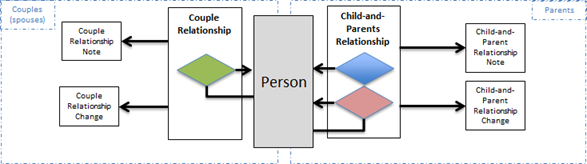
\includegraphics{05/04_relationshipsCore}
        \centering
        \caption{El bloc de l'arbre familiar relatiu a les relacions}\label{img:relationshipsBloc}
    \end{figure}

    Podreu observar també, a les taules que representen l'estructura dels recursos, que a vegades, per la columna que marca el format de dades d'un paràmetre, aquest es troba especificat entre els caràcters `[' i `]'. Aquesta terminologia s'utilitza per indicar que aquest paràmetre és en realitat un recurs o objecte de dades diferent inclòs dins del recurs estudiat.

    També s'observarà que sovint, els recursos exposats, hereten dades d'altres recursos i en els casos que aquests siguin rellevants, se n'exposarà l'estructura a l'apartat `Altres recursos interessants', més endavant en la memòria.

    \subsection{El recurs Relació (Relationship)}

    \paragraph{}
    Aquest recurs s'utilitza en l'actualitat per representar només les relacions de pa\-re\-lla. En el passat, també va ser utilitzat per representar relacions entre pares i fills, mitjançant l'ús del paràmetre \emph{type} i l'enumeració \emph{relationshipType}. Tanmateix, aquest ha caigut en el desús des de la incorporació del recurs Relacions Pares i Fill.

    Aquest recurs emmagatzema informació sobre les persones que conformen la relació de parella i els esdeveniments relacionats a aquesta. Les dades pròpies del recurs es mostren a la taula~\ref{res:relationship} i també hereta les dades dels recursos Subjecte, Conclusió, Enllaços Hypermedia i Dades Extensibles que poden ser trobats a l'apartat `Altres recursos interessants'.

    \begin{center}
             \csvreader[
                separator=comma,
                before table=\sffamily\small,
                longtable={p{2cm-2\tabcolsep}p{3.5cm-2\tabcolsep}p{8.5cm-2\tabcolsep}},
                table head={\caption{Paràmetres del recurs Relació}\label{res:relationship}\\\toprule%
                    \headentry{m{2cm-2\tabcolsep}}{Paràmetre}
                    & \headentry{m{3.4cm-2\tabcolsep}}{Format de Dades}
                    & \headentry{m{8.5cm-2\tabcolsep}}{Descripció}\\\midrule},
                late after line=\\\midrule,
                late after last line=\\\bottomrule,
             ]
             {./tables/05/02_relationships/relation.csv}
             {param=\param,format=\format,desc=\desc}
             {\param&\format&\desc}
     \end{center}


    \subsubsection{L'enumeració relationshipType}

    \paragraph{}
    L'enumeració relationshipType segueix l'estructura de definició GEDCOMX. Com a tal, els valors possibles per l'enumeració segueixen la pauta:

    http://gedcomx.org/ + `relationshipType'

    La següent taula mostra els possibles valors per l'enumeració relationshipType, però com ja hem comentat, l'ús del valor \emph{ParentChild}, ja no s'utilitza en favor del nou recurs Relació Pares i Fill.

    \begin{center}
        \csvreader[
           no head,
           separator=comma,
           table head={\caption{Valors possibles per l'enumeració relationshipType}\label{rel:relationshipType}},
           before table=\sffamily\small,
           longtable={|p{3cm}|p{3cm}|},
           column count=4,
           late after head=\\\hline,
           late after line=\\\hline,
           late after last line=\\\hline,
        ]
        {./tables/05/02_relationships/relationshipType.csv}
        {1=\one,2=\two}
        {\one&\two}
    \end{center}

    \subsection{El recurs Relació Pares i Fill (ChildAndParentsRelationship)}

    \paragraph{}
    Com ja hem comentat, aquest recurs s'utilitza per representar les relacions entre dos pares i un fill. Existeix també la possibilitat de deixar un pare sense especificar, permetent així, la introducció de famílies monoparentals en el sistema.

    Aquest recurs conté informació sobre les persones que conformen els rols de pare, mare i fill, així com el conjunt d'esdeveniments relacionats amb el pare i la mare.

    Els paràmetres del recurs són descrits sa la taula~\ref{res:childAndParents} i recordar que també hereta els paràmetres dels recursos Subjecte, Conclusió, Enllaços Hypermedia i Dades Extensibles que poden ser trobats a l'apartat `Altres recursos interessants'.

    \begin{center}
             \csvreader[
                separator=comma,
                before table=\sffamily\small,
                longtable={p{2cm-2\tabcolsep}p{3.5cm-2\tabcolsep}p{8.5cm-2\tabcolsep}},
                table head={\caption{Paràmetres del recurs Relació Pares i Fill}\label{res:childAndParents}\\\toprule%
                    \headentry{m{2cm-2\tabcolsep}}{Paràmetre}
                    & \headentry{m{3.4cm-2\tabcolsep}}{Format de Dades}
                    & \headentry{m{8.5cm-2\tabcolsep}}{Descripció}\\\midrule},
                late after line=\\\midrule,
                late after last line=\\\bottomrule,
             ]
             {./tables/05/02_relationships/parents.csv}
             {param=\param,format=\format,desc=\desc}
             {\param&\format&\desc}
     \end{center}


    \section{Recursos principals del bloc Discussions}

    \paragraph{}
    El recurs principal d'aquest bloc de l'arbre familiar rep el nom de Discussió. Al mateix temps, podem dir que les discussions estan formades principalment per un conjunt de Comentaris.

    Les discussions a FamilySearch són tòpics de discussió introduïts pels usuaris i relacionats a una persona en concret. Com hem esmentat fa un moment, aquestes discussions estan formades per diferents comentaris i també destaca la utilització d'un recurs intermedi que fa de pont, entre les discussions i els recursos de les persones a les quals fan re\-fe\-rèn\-cia, mitjançant enllaços hypermedia.

    El contingut d'aquestes discussions és bastant divers, però generalment són u\-ti\-lit\-za\-des per discutir, entre diferents usuaris, sobre les dades relatives a una persona, l'origen de les fonts de dades i altres aspectes similars.

    La figura~\ref{img:discussionsBloc} mostra com es troben relacionats els recursos que conformen el bloc Discussions.

    \begin{figure}[h]
        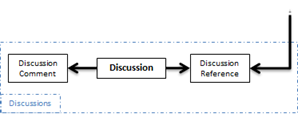
\includegraphics{05/05_discussionsCore}
        \centering
        \caption{El bloc de l'arbre familiar relatiu a les discussions}\label{img:discussionsBloc}
    \end{figure}

    Podreu observar també, a les taules que representen l'estructura dels recursos, que a vegades, per la columna que marca el format de dades d'un paràmetre, aquest es troba especificat entre els caràcters `[' i `]'. Aquesta terminologia s'utilitza per indicar que aquest paràmetre és en realitat un recurs o objecte de dades diferent inclòs dins del recurs estudiat.

    També s'observarà que sovint, els recursos exposats, hereten dades d'altres recursos i en els casos que aquests siguin rellevants, se n'exposarà l'estructura a l'apartat `Altres recursos interessants', més endavant en la memòria.

    \subsection{El recurs Referència a la Discussió (DiscussionsReference)}

    \paragraph{}
    Aquest recurs s'utilitza principalment perquè el recurs Persona puguin accedir al conjunt de discussions que tracten sobre ella i viceversa. En concret, existirà un enllaç per cada una de les discussions que reverenciïn a la mateixa persona.

    Les dades contingudes per aquest recurs poden ser trobades a la taula~\ref{res:discussionReference} i també hereta els paràmetres dels recursos Enllaços Hypermedia i Dades Extensibles que poden ser trobats a l'apartat `Altres recursos interessants'.

    \begin{center}
             \csvreader[
                separator=comma,
                before table=\sffamily\small,
                longtable={p{2cm-2\tabcolsep}p{3.5cm-2\tabcolsep}p{8.5cm-2\tabcolsep}},
                table head={\caption{Paràmetres del recurs Referència a la Discussió}\label{res:discussionReference}\\\toprule%
                    \headentry{m{2cm-2\tabcolsep}}{Paràmetre}
                    & \headentry{m{3.4cm-2\tabcolsep}}{Format de Dades}
                    & \headentry{m{8.5cm-2\tabcolsep}}{Descripció}\\\midrule},
                late after line=\\\midrule,
                late after last line=\\\bottomrule,
             ]
             {./tables/05/03_discussions/discussionReference.csv}
             {param=\param,format=\format,desc=\desc}
             {\param&\format&\desc}
     \end{center}

    \subsection{El recurs Discussió (Discussion)}

    \paragraph{}
    El recurs Discussió és utilitzat per representar el tòpic sobre el qual tractarà la conversació entre els diferents usuaris de FamilySearch i emmagatzemar el conjunt de comentaris introduïts per aquests.

    El recurs Discussió, esdevé un objecte bastant simple, contenint només la informació necessària perquè altres usuaris puguin comprendre el tòpic de discussió, les metadades de la creació i accedir al conjunt de comentaris.

    Aquest recurs està format pels paràmetres mostrats a la taula~\ref{res:discussion} i també hereta els paràmetres dels recursos Enllaços Hypermedia i Dades Extensibles, que poden ser trobats a l'apartat `Altres recursos interessants'.

    \begin{center}
             \csvreader[
                separator=semicolon,
                before table=\sffamily\small,
                longtable={p{2cm-2\tabcolsep}p{3.5cm-2\tabcolsep}p{8.5cm-2\tabcolsep}},
                table head={\caption{Paràmetres del recurs Discussió}\label{res:discussion}\\\toprule%
                    \headentry{m{2cm-2\tabcolsep}}{Paràmetre}
                    & \headentry{m{3.4cm-2\tabcolsep}}{Format de Dades}
                    & \headentry{m{8.5cm-2\tabcolsep}}{Descripció}\\\midrule},
                late after line=\\\midrule,
                late after last line=\\\bottomrule,
             ]
             {./tables/05/03_discussions/discussion.csv}
             {param=\param,format=\format,desc=\desc}
             {\param&\format&\desc}
     \end{center}

    \subsection{El recurs Comentari (Comment)}

    \paragraph{}
    El recurs Comentari conté els missatges introduïts pels diferents usuaris com a resposta a una discussió. Principalment, conté informació sobre la data de creació, l'usuari que l'ha enviat i el text en qüestió propi del comentari.

    Les dades pròpies d'aquest recurs es mostren a la taula~\ref{res:comment} i també hereta els paràmetres dels recursos Enllaços Hypermedia i Dades Extensibles que poden ser trobats a l'apartat `Altres recursos interessants'.

    \begin{center}
             \csvreader[
                separator=comma,
                before table=\sffamily\small,
                longtable={p{2cm-2\tabcolsep}p{3.5cm-2\tabcolsep}p{8.5cm-2\tabcolsep}},
                table head={\caption{Paràmetres del recurs Comentari}\label{res:comment}\\\toprule%
                    \headentry{m{2cm-2\tabcolsep}}{Paràmetre}
                    & \headentry{m{3.4cm-2\tabcolsep}}{Format de Dades}
                    & \headentry{m{8.5cm-2\tabcolsep}}{Descripció}\\\midrule},
                late after line=\\\midrule,
                late after last line=\\\bottomrule,
             ]
             {./tables/05/03_discussions/comment.csv}
             {param=\param,format=\format,desc=\desc}
             {\param&\format&\desc}
     \end{center}


    \section{Recursos principals del bloc Memòries}

    \paragraph{}
    El bloc Memòries és relativament nou a l'API de FamilySearch i la documentació al respecte és pràcticament inexistent. Aquest bloc conté les memòries penjades al núvol pels usuaris i són relacionades amb les persones de l'arbre familiar.

    Recordem, que el concepte memòries ha estat descrit a la secció tres de la memòria, `L'organització Familysearch' i consisteixen principalment en contingut fotogràfic, històries, documents diversos i fitxers d'àudio.

    El recurs principal d'aquest bloc és el recurs Memòria, que conté tota la informació específica d'aquesta. Les memòries també contenen comentaris, en un estil molt similar a les discussions i també disposen de recursos intermedis per relacionar les memòries amb les persones a les quals fan referència. Com sempre, moltes d'aquestes connexions són implementades a través d'enllaços hypermedia.

    De moment, resulta necessari crear una instància del recurs Memòria per cada contingut que es vulgui pujar al sistema, però la possibilitat de suportar més d'un artefacte amb el mateix recurs memòria ha estat estudiat i en algun moment o altre serà implementat. Un exemple  de cas d'ús podria ser la necessitat de pujar les dues cares d'una fotografia.

    La imatge~\ref{img:memoriesBloc} ofereix un esquema de forma visual de com es relacionen els recursos vinculats al bloc Memòries.

    \begin{figure}[h]
        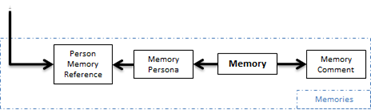
\includegraphics{05/06_memoriesCore}
        \centering
        \caption{El bloc de l'arbre familiar relatiu a les memòries}\label{img:memoriesBloc}
    \end{figure}

    Desgraciadament, la documentació referent a aquest apartat per part de FamilySearch és molt pobre i el contingut de cada un dels recursos ha estat creat per inferència mitjançant el collage de petites peces d'informació i les similituds que presentaven amb altres recursos similars de l'API. És possible que els recursos presentats a continuació no descriguin amb total precisió la realitat exacta.

    Podreu observar també, a les taules que representen l'estructura dels recursos, que a vegades, per la columna que marca el format de dades d'un paràmetre, aquest es troba especificat entre els caràcters `[' i `]'. Aquesta terminologia s'utilitza per indicar que aquest paràmetre és en realitat un recurs o objecte de dades diferent inclòs dins del recurs estudiat.

    També s'observarà que sovint, els recursos exposats, hereten dades d'altres recursos i en els casos que aquests siguin rellevants, se n'exposarà l'estructura a l'apartat `Altres recursos interessants', més endavant en la memòria.

    \subsection{El recurs Referència a la Memòria d'una Persona (Person Memory Reference)}

    \paragraph{}
    Aquest recurs és utilitzat com a pont entre el recurs Persona i el contingut específic de les memòries. Existirà un enllaç hypermedia diferent per cada una de les memòries a les quals el recurs Persona hagi de tenir accés i viceversa.

    Les dades contingudes per aquest recurs poder ser trobades a la taula~\ref{res:memoryReference} i també hereta els paràmetres dels recursos Enllaços Hypermedia i Dades Extensibles, que poden ser trobats a l'apartat `Altres recursos interessants'.

    \begin{center}
             \csvreader[
                separator=comma,
                before table=\sffamily\small,
                longtable={p{2cm-2\tabcolsep}p{3.5cm-2\tabcolsep}p{8.5cm-2\tabcolsep}},
                table head={\caption{Paràmetres del recurs Referència a la Memòria}\label{res:memoryReference}\\\toprule%
                    \headentry{m{2cm-2\tabcolsep}}{Paràmetre}
                    & \headentry{m{3.4cm-2\tabcolsep}}{Format de Dades}
                    & \headentry{m{8.5cm-2\tabcolsep}}{Descripció}\\\midrule},
                late after line=\\\midrule,
                late after last line=\\\bottomrule,
             ]
             {./tables/05/04_memories/memoryReference.csv}
             {param=\param,format=\format,desc=\desc}
             {\param&\format&\desc}
     \end{center}

    \subsection{El recurs Persones en una Memòria (MemoryPersona)}

    \paragraph{}
    Aquest recurs s'utilitza com a pont per accedir a totes les persones que han estat marcades com a relacionades en una memòria. Per exemple, si una fotografia conté la imatge de diverses persones i es vol relacionar la memòria amb totes elles, aquest recurs ho fa possible sense la necessitat d'haver de pujar la imatge per cada usuari.

    La taula~\ref{res:memoryPersona} mostra els paràmetres d'aquest recurs, que també hereta els paràmetres dels recursos Enllaços Hypermedia i Dades Extensibles, que poden ser trobats a l'apartat `Altres recursos interessants'.

    \begin{center}
             \csvreader[
                separator=comma,
                before table=\sffamily\small,
                longtable={p{2cm-2\tabcolsep}p{3.5cm-2\tabcolsep}p{8.5cm-2\tabcolsep}},
                table head={\caption{Paràmetres del recurs Persones en una memòria}\label{res:memoryPersona}\\\toprule%
                    \headentry{m{2cm-2\tabcolsep}}{Paràmetre}
                    & \headentry{m{3.4cm-2\tabcolsep}}{Format de Dades}
                    & \headentry{m{8.5cm-2\tabcolsep}}{Descripció}\\\midrule},
                late after line=\\\midrule,
                late after last line=\\\bottomrule,
             ]
             {./tables/05/04_memories/memoryPersona.csv}
             {param=\param,format=\format,desc=\desc}
             {\param&\format&\desc}
     \end{center}

    \subsection{El recurs Memòria (Memory)}

    \paragraph{}
    El recurs Memòria, com el seu nom indica, és el recurs principal utilitzat per emmagatzemar la informació relacionada a un artefacte pujat per un usuari. Per fer-ho, s'utilitza el recurs Descripció de la Font de Dades, que s'especificarà més endavant, a l'apartat de recursos relacionats amb el bloc Fonts de Dades.

    Aquest recurs també inclou instàncies dels comentaris que han estat associats a les memòries.

    Els paràmetres d'aquest recurs es mostren a la taula~\ref{res:memory} i també hereta els paràmetres dels recursos Enllaços Hypermedia i Dades Extensibles, que poden ser trobats a l'apartat `Altres recursos interessants'.

    \begin{center}
             \csvreader[
                separator=semicolon,
                before table=\sffamily\small,
                longtable={p{2cm-2\tabcolsep}p{3.5cm-2\tabcolsep}p{8.5cm-2\tabcolsep}},
                table head={\caption{Paràmetres del recurs Memòria}\label{res:memory}\\\toprule%
                    \headentry{m{2cm-2\tabcolsep}}{Paràmetre}
                    & \headentry{m{3.4cm-2\tabcolsep}}{Format de Dades}
                    & \headentry{m{8.5cm-2\tabcolsep}}{Descripció}\\\midrule},
                late after line=\\\midrule,
                late after last line=\\\bottomrule,
             ]
             {./tables/05/04_memories/memory.csv}
             {param=\param,format=\format,desc=\desc}
             {\param&\format&\desc}
     \end{center}


    \section{Recursos principals del bloc Fonts de Dades}

    \paragraph{}
    Aquest bloc de l'arbre familiar destaca pels recursos Col·lecció i Font de Dades, utilitzats per certificar la veracitat de les dades genealògiques relacionades a les persones de l'arbre familiar o a les relacions que les uneixen.

    Aquest bloc és realment important, ja que és l'encarregat de garantir la integritat de les dades i per tant, d'assegurar que la informació continguda a l'arbre familiar de FamilySearch sigui usable i interessant pels usuaris de l'aplicació.

    Així doncs, les fonts de dades són utilitzades per demostrar que un esdeveniment en concret va succeir o que les dades de la persona citada són les mateixes que aquelles redactades en els documents oficials.

    Les fonts de dades s'agrupen i emmagatzemen en col·leccions i cada persona o relació, disposa d'un recurs que actua com intermediari per relacionar-los amb les fonts de dades. Com sempre, els enllaços explícits entre els diferents recursos es realitzen mitjançant els enllaços hypermedia. La imatge~\ref{img:sourcesBloc} ofereix una vista de com s'estructuren i relacionen els diferents recursos del bloc Font de Dades.

    \begin{figure}[h]
        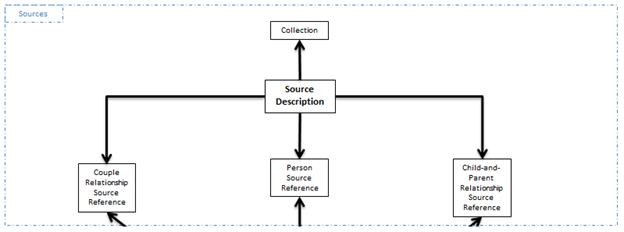
\includegraphics{05/07_sourcesCore}
        \centering
        \caption{El bloc de l'arbre familiar relatiu a les fonts de dades}\label{img:sourcesBloc}
    \end{figure}

    Podreu observar també, a les taules que representen l'estructura dels recursos, que a vegades, per la columna que marca el format de dades d'un paràmetre, aquest es troba especificat entre els caràcters `[' i `]'. Aquesta terminologia s'utilitza per indicar que aquest paràmetre és en realitat un recurs o objecte de dades diferent inclòs dins del recurs estudiat.

    També s'observarà que sovint, els recursos exposats, hereten dades d'altres recursos i en els casos que aquests siguin rellevants, se n'exposarà l'estructura a l'apartat `Altres recursos interessants', més endavant en la memòria.

    \subsection{El recurs Col·lecció (Collection)}

    \paragraph{}
    Aquest recurs representa una col·lecció o agregació, de fonts de dades de caràcter genealògic.

    Aquestes dades poden fer referència tant a les dades internes de FamilySearch, com als registres bolcats per tercers a les bases de dades. Per tal d'ajudar al lector a fer-se una idea, una col·lecció podria ser per exemple el conjunt de fonts de dades que conformen l'arbre familiar.

    La taula~\ref{res:collection} mostra els paràmetres que aquest recurs incorpora i també hereta els paràmetres dels recursos Enllaços Hypermedia i Dades Extensibles que poden ser trobats a l'apartat `Altres recursos interessants'.

    \begin{center}
             \csvreader[
                separator=comma,
                before table=\sffamily\small,
                longtable={p{2cm-2\tabcolsep}p{3.5cm-2\tabcolsep}p{8.5cm-2\tabcolsep}},
                table head={\caption{Paràmetres del recurs Col·lecció}\label{res:collection}\\\toprule%
                    \headentry{m{2cm-2\tabcolsep}}{Paràmetre}
                    & \headentry{m{3.4cm-2\tabcolsep}}{Format de Dades}
                    & \headentry{m{8.5cm-2\tabcolsep}}{Descripció}\\\midrule},
                late after line=\\\midrule,
                late after last line=\\\bottomrule,
             ]
             {./tables/05/05_sources/collection.csv}
             {param=\param,format=\format,desc=\desc}
             {\param&\format&\desc}
     \end{center}

    \subsection{El recurs Contingut de la Col·lecció (CollectionContent)}

    \paragraph{}
    Aquest recurs conté informació específica sobre la col·lecció a la que fa referència. Serveix per  comprendre millor l'estat actual de migració de la col·lecció a les bases de dades de FamilySearch, així com informació sobre el contingut que aquesta aporta.

    La taula~\ref{res:collectionContent} mostra els paràmetres inclosos en el recurs, que a la vegada hereta els paràmetres dels recursos Enllaços Hypermedia i Dades Extensibles que poden ser trobats a l'apartat `Altres recursos interessants'.

    \begin{center}
             \csvreader[
                separator=comma,
                before table=\sffamily\small,
                longtable={p{2cm-2\tabcolsep}p{3.5cm-2\tabcolsep}p{8.5cm-2\tabcolsep}},
                table head={\caption{Paràmetres del recurs Contingut de la Col·lecció}\label{res:collectionContent}\\\toprule%
                    \headentry{m{2cm-2\tabcolsep}}{Paràmetre}
                    & \headentry{m{3.4cm-2\tabcolsep}}{Format de Dades}
                    & \headentry{m{8.5cm-2\tabcolsep}}{Descripció}\\\midrule},
                late after line=\\\midrule,
                late after last line=\\\bottomrule,
             ]
             {./tables/05/05_sources/collectionContent.csv}
             {param=\param,format=\format,desc=\desc}
             {\param&\format&\desc}
     \end{center}

    \subsection{El recurs Atribució (Attribution)}

    \paragraph{}
    El recurs Atribució s'utilitza en més llocs que les fonts de dades, però com que juga un paper especialment important en aquest, hem decidit incloure'l dins d'aquesta secció.

    Aquest recurs conté principalment paràmetres que permeten descriure qui, quan i perquè, va ser realitzada una contribució o modificació sobre les dades.

    Els paràmetres d'aquest recurs són descrits a la taula~\ref{res:attribution}, que també hereta els paràmetres del recurs Dades Extensibles, que pot ser trobat a l'apartat `Altres recursos interessants'.

    \begin{center}
             \csvreader[
                separator=comma,
                before table=\sffamily\small,
                longtable={p{2cm-2\tabcolsep}p{3.5cm-2\tabcolsep}p{8.5cm-2\tabcolsep}},
                table head={\caption{Paràmetres del recurs Atribució}\label{res:attribution}\\\toprule%
                    \headentry{m{2cm-2\tabcolsep}}{Paràmetre}
                    & \headentry{m{3.4cm-2\tabcolsep}}{Format de Dades}
                    & \headentry{m{8.5cm-2\tabcolsep}}{Descripció}\\\midrule},
                late after line=\\\midrule,
                late after last line=\\\bottomrule,
             ]
             {./tables/05/05_sources/attribution.csv}
             {param=\param,format=\format,desc=\desc}
             {\param&\format&\desc}
     \end{center}

    \subsection{El recurs Font de Dades (SourceDescription)}

    \paragraph{}
    Aquest recurs defineix una font de dades i n'emmagatzema tota la informació que la caracteritza. Les fonts de dades formen part d'una col·lecció i es troben relacionades a ella mitjançant enllaços hypermedia.

    La millor forma d'explicar aquest recurs és comprendre'n els paràmetres i aquests s'exposen a la taula~\ref{res:sourceDescription}. El recurs Font de Dades també hereta els paràmetres dels recursos Enllaços Hypermedia i Dades Extensibles, que poden ser trobats a l'apartat `Altres recursos interessants'.

    \begin{center}
             \csvreader[
                separator=semicolon,
                before table=\sffamily\small,
                longtable={p{2cm-2\tabcolsep}p{3.5cm-2\tabcolsep}p{8.5cm-2\tabcolsep}},
                table head={\caption{Paràmetres del recurs Font de Dades}\label{res:sourceDescription}\\\toprule%
                    \headentry{m{2cm-2\tabcolsep}}{Paràmetre}
                    & \headentry{m{3.4cm-2\tabcolsep}}{Format de Dades}
                    & \headentry{m{8.5cm-2\tabcolsep}}{Descripció}\\\midrule},
                late after line=\\\midrule,
                late after last line=\\\bottomrule,
             ]
             {./tables/05/05_sources/sourceDescription.csv}
             {param=\param,format=\format,desc=\desc}
             {\param&\format&\desc}
     \end{center}


    \subsubsection{L'enumeració resourceType}

    L'enumeració resourceType segueix l'estructura de definició GEDCOMX. Com a tal, els valors possibles per l'enumeració segueixen la pauta:

    http://gedcomx.org/ + `resourceType'

    La següent taula mostra els possibles valors per l'enumeració resourceType.

    \begin{center}
        \csvreader[
           no head,
           separator=comma,
           table head={\caption{Valors possibles per l'enumeració resourceType}\label{enum:resourceType}},
           before table=\sffamily\small,
           longtable={|p{3cm}|p{3cm}|p{3cm}|},
           column count=3,
           late after head=\\\hline,
           late after line=\\\hline,
           late after last line=\\\hline,
        ]
        {./tables/05/05_sources/resourceType.csv}
        {1=\one,2=\two,3=\three}
        {\one&\two&\three}
    \end{center}

    \subsection{El recurs Referència a la Font de Dades (SourceReference)}

    \paragraph{}
    Aquest recurs s'utilitza per fer de pont entre els diferents recursos de l'arbre fa\-mi\-liar, que contenen informació genealògica i les fonts de dades que l'han proporcionat.

    Com s'ha pogut veure en la imatge~\ref{img:sourcesBloc}, que obria el bloc de Fonts de Dades, el recurs Referència a la Font de Dades aplica tant a les relacions familiars, com a les persones. De la mateixa forma, aquest recurs també es veu utilitzat per relacionar diferents Fonts de Dades entre elles.

    A part dels paràmetres que conformen aquest recurs i que es mostren a la taula~\ref{res:sourceReference}, també hereta els paràmetres dels recursos Enllaços Hypermedia i Dades Extensibles, que poden ser trobats a l'apartat `Altres recursos interessants'.

    \begin{center}
             \csvreader[
                separator=semicolon,
                before table=\sffamily\small,
                longtable={p{2cm-2\tabcolsep}p{3.5cm-2\tabcolsep}p{8.5cm-2\tabcolsep}},
                table head={\caption{Recurs Referència a la Font de Dades}\label{res:sourceReference}\\\toprule%
                    \headentry{m{2cm-2\tabcolsep}}{Paràmetre}
                    & \headentry{m{3.4cm-2\tabcolsep}}{Format de Dades}
                    & \headentry{m{8.5cm-2\tabcolsep}}{Descripció}\\\midrule},
                late after line=\\\midrule,
                late after last line=\\\bottomrule,
             ]
             {./tables/05/05_sources/sourceReference.csv}
             {param=\param,format=\format,desc=\desc}
             {\param&\format&\desc}
     \end{center}


    \section{Altres recursos interessants}

    \paragraph{}
    Com haureu pogut observar després de la lectura de les seccions anteriors, no tots els objectes o recursos que han anat apareixent com a paràmetres dels recursos estudiants, han estat descrits en profunditat. Les raons són diverses segons el recurs en qüestió, però alguns motius comuns són els següents:

    \begin{itemize}
        \item És un recurs orientat a la manipulació de les dades, més que a proporcionar informació genealògica a l'usuari i per tant, no acaba de prendre valor per l'estudi realitzat en els apartats anteriors.
        \item Es tracta d'un recurs simple del qual no s'aportaria més informació mostrant-ne l'estructura, que simplement disposant de la descripció del camp.
        \item És un recurs utilitzat en cassos molt específics i per tant, no aplicable en un àmbit general.
    \end{itemize}

    Això no obstant, sí que hi ha altres recursos que s'han vist representats a les seccions anteriors de forma transversal i que volem explicar. Exemples d'aquests recursos són les Notes i els històrics de Canvis, que per exemple, podien ser trobats en les imatges que unien els recursos de cada bloc.

    També existeix un conjunt de recursos que hem anat mencionant en els apartats anteriors, on els recursos estudiats heretaven els paràmetres d'aquests. Aquests recursos incorporats de forma global a molts altres, també seran estudiats en aquest apartat de la memòria.

    A part d'aquests dos grups de recursos, també volem descriure'n d'altres que considerem que sota certes circumstàncies podrien resultar interessants i encara que no s'han vist relacionats de forma directa amb els blocs de dades anteriors, volem deixar-ne constància en el projecte.

    \subsection{El recurs Subjecte (Subject)}

    \paragraph{}
    El recurs Subjecte fa referència al concepte abstracte de subjecte genealògic, entenent-lo com una entitat única que o bé pot fer referència a una persona o a una localització concreta del globus terraqüi.

    Aquesta entitat única, agrega i emmagatzema les diferents evidències i fonts de dades particulars del subjecte, és a dir, el col·lectiu d'informació que fan que aquest subjecte sigui diferent dels altres.

    La taula~\ref{res:subject} mostra al que ens referim quan parlem d'aquesta agregació d'infor\-mació.

    \clearpage

    \begin{center}
             \csvreader[
                separator=comma,
                before table=\sffamily\small,
                longtable={p{2cm-2\tabcolsep}p{3.5cm-2\tabcolsep}p{8.5cm-2\tabcolsep}},
                table head={\caption{Paràmetres del recurs Subjecte}\label{res:subject}\\\toprule%
                    \headentry{m{2cm-2\tabcolsep}}{Paràmetre}
                    & \headentry{m{3.4cm-2\tabcolsep}}{Format de Dades}
                    & \headentry{m{8.5cm-2\tabcolsep}}{Descripció}\\\midrule},
                late after line=\\\midrule,
                late after last line=\\\bottomrule,
             ]
             {./tables/05/06_others/subject.csv}
             {param=\param,format=\format,desc=\desc}
             {\param&\format&\desc}
     \end{center}

    \subsection{El recurs Conclusió (Conclusion)}

    \paragraph{}
    En l'àmbit de l'API de FamilySearch, el terme conclusió fa referència al valor que pren una dada genealògica després de ser contrastada amb una font de dades. És doncs, l'avaluació del valor que certa dada genealògica o conjunt de dades genealògiques, han rebut.

    Aquest recurs conté els paràmetres que s'expressen a la taula~\ref{res:conclusion}.

    \begin{center}
             \csvreader[
                separator=comma,
                before table=\sffamily\small,
                longtable={p{2cm-2\tabcolsep}p{3.5cm-2\tabcolsep}p{8.5cm-2\tabcolsep}},
                table head={\caption{Paràmetres del recurs Conclusió}\label{res:conclusion}\\\toprule%
                    \headentry{m{2cm-2\tabcolsep}}{Paràmetre}
                    & \headentry{m{3.4cm-2\tabcolsep}}{Format de Dades}
                    & \headentry{m{8.5cm-2\tabcolsep}}{Descripció}\\\midrule},
                late after line=\\\midrule,
                late after last line=\\\bottomrule,
             ]
             {./tables/05/06_others/conclusion.csv}
             {param=\param,format=\format,desc=\desc}
             {\param&\format&\desc}
     \end{center}

    \subsection{El recurs Enllaços Hypermedia (Hypermedia Enabled Data)}

    \paragraph{}
    Aquest recurs es troba en pràcticament tots els altres recursos de l'API de Family\-Search. Són els responsables de poder navegar a través dels diferents recursos que es troben relacionats en el model de dades de FamilySearch, sense necessitat de codificar noves URIs de forma manual o des d'una aplicació.

    Aquest recurs consisteix bàsicament en un conjunt d'enllaços que apunten als diferents recursos. La taula~\ref{res:hypermedia} en mostra l'estructura en detall.

    \begin{center}
             \csvreader[
                separator=comma,
                before table=\sffamily\small,
                longtable={p{2cm-2\tabcolsep}p{3.5cm-2\tabcolsep}p{8.5cm-2\tabcolsep}},
                table head={\caption{Paràmetres del recurs Enllaços Hypermedia}\label{res:hypermedia}\\\toprule%
                    \headentry{m{2cm-2\tabcolsep}}{Paràmetre}
                    & \headentry{m{3.4cm-2\tabcolsep}}{Format de Dades}
                    & \headentry{m{8.5cm-2\tabcolsep}}{Descripció}\\\midrule},
                late after line=\\\midrule,
                late after last line=\\\bottomrule,
             ]
             {./tables/05/06_others/hypermedia.csv}
             {param=\param,format=\format,desc=\desc}
             {\param&\format&\desc}
     \end{center}

    \subsection{El recurs Enllaç (Link)}

    \paragraph{}
    A diferència del que es pugui creure, en el context de l'API de FamilySearch, Link no fa referència al famós protagonista de la saga de videojocs `Zelda', sinó a un enllaç hypermedia com el descrit en els començaments d'aquesta secció de la memòria.

    Com ja s'ha comentat nombroses vegades, aquests enllaços existeixen per facilitar la navegació entre recursos. L'estructura del recurs Enllaç pot veure's en detall a la taula~\ref{res:link}.

    \begin{center}
             \csvreader[
                separator=comma,
                before table=\sffamily\small,
                longtable={p{2cm-2\tabcolsep}p{3.5cm-2\tabcolsep}p{8.5cm-2\tabcolsep}},
                table head={\caption{Paràmetres del recurs Enllaç}\label{res:link}\\\toprule%
                    \headentry{m{2cm-2\tabcolsep}}{Paràmetre}
                    & \headentry{m{3.4cm-2\tabcolsep}}{Format de Dades}
                    & \headentry{m{8.5cm-2\tabcolsep}}{Descripció}\\\midrule},
                late after line=\\\midrule,
                late after last line=\\\bottomrule,
             ]
             {./tables/05/06_others/link.csv}
             {param=\param,format=\format,desc=\desc}
             {\param&\format&\desc}
     \end{center}

    \subsection{El recurs Dades Extensibles (Extensible Data)}

    \paragraph{}
    Aquest recurs és probablement el més simple de tots. S'encarrega de dotar a tots els altres recursos de l'API de FamilySearch, amb un identificador local únic, que permeti referenciar-lo a les bases de dades.

    La taula~\ref{res:extensibleData} mostra l'estructura d'aquest recurs.

    \begin{center}
             \csvreader[
                separator=comma,
                before table=\sffamily\small,
                longtable={p{2cm-2\tabcolsep}p{3.5cm-2\tabcolsep}p{8.5cm-2\tabcolsep}},
                table head={\caption{Paràmetres del recurs Dades Extensibles}\label{res:extensibleData}\\\toprule%
                    \headentry{m{2cm-2\tabcolsep}}{Paràmetre}
                    & \headentry{m{3.4cm-2\tabcolsep}}{Format de Dades}
                    & \headentry{m{8.5cm-2\tabcolsep}}{Descripció}\\\midrule},
                late after line=\\\midrule,
                late after last line=\\\bottomrule,
             ]
             {./tables/05/06_others/extensibleData.csv}
             {param=\param,format=\format,desc=\desc}
             {\param&\format&\desc}
     \end{center}

    \subsection{El recurs Nota (Note)}

    \paragraph{}
    Aquest recurs pot ser vinculat a persones, relacions i fonts de dades. És un recurs utilitzat per realitzar alguna anotació específica sobre les dades a les quals ha estat relacionat.

    El recurs Nota també hereta els paràmetres dels recursos Enllaços Hypermedia i Dades Extensibles, que poden trobar-se en aquest mateix apartat de la memòria i té per paràmetres propis els que es mostren a la taula~\ref{res:note}.

    \begin{center}
             \csvreader[
                separator=comma,
                before table=\sffamily\small,
                longtable={p{2cm-2\tabcolsep}p{3.5cm-2\tabcolsep}p{8.5cm-2\tabcolsep}},
                table head={\caption{Paràmetres del recurs Nota}\label{res:note}\\\toprule%
                    \headentry{m{2cm-2\tabcolsep}}{Paràmetre}
                    & \headentry{m{3.4cm-2\tabcolsep}}{Format de Dades}
                    & \headentry{m{8.5cm-2\tabcolsep}}{Descripció}\\\midrule},
                late after line=\\\midrule,
                late after last line=\\\bottomrule,
             ]
             {./tables/05/06_others/note.csv}
             {param=\param,format=\format,desc=\desc}
             {\param&\format&\desc}
     \end{center}

    \subsection{El recurs Referència al Recurs (ResourceReference)}

    \paragraph{}
    Un altre recurs que ha sortit molt fins ara, com a recurs contingut dins dels altres recursos, és el de Referència al Recurs. Aquest objecte, s'utilitza per enllaçar mitjançant un contingut semàntic, representat per l'identificador del camp del recurs apuntat i la seva URI, un recurs amb un altre.

    El seu format és molt simple i consta només dels dos paràmetres exposats a la taula~\ref{res:resourceReference}.

    \begin{center}
             \csvreader[
                separator=comma,
                before table=\sffamily\small,
                longtable={p{2cm-2\tabcolsep}p{3.5cm-2\tabcolsep}p{8.5cm-2\tabcolsep}},
                table head={\caption{Paràmetres del recurs Referència al Recurs}\label{res:resourceReference}\\\toprule%
                    \headentry{m{2cm-2\tabcolsep}}{Paràmetre}
                    & \headentry{m{3.4cm-2\tabcolsep}}{Format de Dades}
                    & \headentry{m{8.5cm-2\tabcolsep}}{Descripció}\\\midrule},
                late after line=\\\midrule,
                late after last line=\\\bottomrule,
             ]
             {./tables/05/06_others/resourceReference.csv}
             {param=\param,format=\format,desc=\desc}
             {\param&\format&\desc}
     \end{center}

    \subsection{El recurs Usuari (User)}\label{sec:user}

    \paragraph{}
    El recurs Usuari conté tota la informació relacionada a l'usuari que es troba identificat amb l'aplicació FamilySearch.

    Aquesta informació pot resultar d'interès per les interfícies d'usuari de les aplicacions, en cas de desitjar realitzar alguna mena de personalització del contingut. El recurs també pot ser utilitzat per accedir a l'arbre genealògic de l'usuari o al recurs de la seva persona a l'arbre familiar.

     Aquest recurs, com molts altres que ja hem exposat, també hereta els paràmetres dels recursos Enllaços Hypermedia i Dades Extensibles, que poden trobar-se en aquest mateix apartat de la memòria i té, per paràmetres propis, els que es mostren a la taula~\ref{res:user}.

     \begin{center}
              \csvreader[
                 separator=comma,
                 before table=\sffamily\small,
                 longtable={p{4cm-2\tabcolsep}p{2cm-2\tabcolsep}p{8cm-2\tabcolsep}},
                 table head={\caption{Paràmetres del recurs Usuari}\label{res:user}\\\toprule%
                     \headentry{m{4cm-2\tabcolsep}}{Paràmetre}
                     & \headentry{m{2cm-2\tabcolsep}}{Format de Dades}
                     & \headentry{m{8cm-2\tabcolsep}}{Descripció}\\\midrule},
                 late after line=\\\midrule,
                 late after last line=\\\bottomrule,
              ]
              {./tables/05/06_others/user.csv}
              {param=\param,format=\format,desc=\desc}
              {\param&\format&\desc}
      \end{center}

    \subsection{El recurs Canvi (Change)}

    \paragraph{}
    Un altre recurs transversal, per alguns dels recursos més importants de l'API de FamilySearch, és el recurs Canvi.

    Quan un usuari realitza alguna modificació de qualsevol mena, ja sigui sobre la informació d'una persona o sobre una relació de parella o parental, aquest canvi queda enregistrat per diversos motius.

    El primer, poder veure com les dades s'han anat modificat al llarg del temps i observar-ne la progressió. El segon, poder recuperar un estat anterior en cas d'error o problema en el sistema.

    El recurs Canvi està format pels paràmetres mostrats a la taula~\ref{res:change}.

    \begin{center}
             \csvreader[
                separator=semicolon,
                before table=\sffamily\small,
                longtable={p{2cm-2\tabcolsep}p{3.5cm-2\tabcolsep}p{8.5cm-2\tabcolsep}},
                table head={\caption{Paràmetres del recurs Canvi}\label{res:change}\\\toprule%
                    \headentry{m{2cm-2\tabcolsep}}{Paràmetre}
                    & \headentry{m{3.4cm-2\tabcolsep}}{Format de Dades}
                    & \headentry{m{8.5cm-2\tabcolsep}}{Descripció}\\\midrule},
                late after line=\\\midrule,
                late after last line=\\\bottomrule,
             ]
             {./tables/05/06_others/change.csv}
             {param=\param,format=\format,desc=\desc}
             {\param&\format&\desc}
     \end{center}


     \subsubsection{L'enumeració changeObjectModifier}

     \paragraph{}
     L'enumeració changeObjectModifier segueix l'estructura de definició GEDCOMX. Com a tal, els valors possibles per l'enumeració segueixen la pauta:

     verb|http://gedcomx.org/ + `changeObjectModifier'

     La taula~\ref{enum:changeObjectModifier} mostra els possible valors de l'enumeració changeObject\-Modifier.

     \begin{center}
         \csvreader[
            no head,
            separator=comma,
            table head={\caption{Valors possibles per l'enumeració changeObjectModifier}\label{enum:changeObjectModifier}},
            before table=\sffamily\small,
            longtable={|p{3cm}|p{3cm}|p{6cm}|},
            column count=4,
            late after head=\\\hline,
            late after line=\\\hline,
            late after last line=\\\hline,
         ]
         {./tables/05/06_others/changeObjectModifier.csv}
         {1=\one,2=\two,3=\three}
         {\one&\two&\three}
     \end{center}


     \subsubsection{L'enumeració changeOperation}

     \paragraph{}
     L'enumeració changeOperation segueix l'estructura de definició GEDCOMX. Com a tal, els valors possibles per l'enumeració segueixen la pauta:

     http://gedcomx.org/ + `changeOperation'

     La taula~\ref{enum:changeOperation} mostra els possibles valors de l'enumeració changeOperation.

     \begin{center}
         \csvreader[
            no head,
            separator=comma,
            table head={\caption{Valors possibles per l'enumeració changeOperation}\label{enum:changeOperation}},
            before table=\sffamily\small,
            longtable={|p{3cm}|p{3cm}|p{3cm}|p{3cm}|},
            column count=4,
            late after head=\\\hline,
            late after line=\\\hline,
            late after last line=\\\hline,
         ]
         {./tables/05/06_others/changeOperation.csv}
         {1=\one,2=\two,3=\three,4=\four}
         {\one&\two&\three&\four}
     \end{center}


     \subsubsection{L'enumeració changeObjectType}

     \paragraph{}
     L'enumeració changeObjectType segueix l'estructura de definició GEDCOMX. Com a tal, els valors possibles per l'enumeració segueixen la pauta:

     http://gedcomx.org/ + `changeObjectType'

     La taula~\ref{enum:changeObjectType} mostra els possibles valors de l'enumeració changeObjectType.

     \begin{center}
         \csvreader[
            no head,
            separator=comma,
            table head={\caption{Valors possibles per l'enumeració changeObjectType}\label{enum:changeObjectType}},
            before table=\sffamily\small,
            longtable={|p{3cm}|p{3cm}|p{3cm}|p{3cm}|},
            column count=4,
            late after head=\\\hline,
            late after line=\\\hline,
            late after last line=\\\hline,
         ]
         {./tables/05/06_others/changeObjectType.csv}
         {1=\one,2=\two,3=\three,4=\four}
         {\one&\two&\three&\four}
     \end{center}

    \subsection{El recurs Agent (Agent)}

    \paragraph{}
    El recurs agent representa a una persona, organització o col·lectiu. En la recerca genealògica, un Agent, generalment pren el rol de contribuïdor.

    La gran majoria dels paràmetres de contribuïdors que ens hem anat trobant fins ara en els diferents recursos, apunten a una instància del recurs Agent.

    Aquest recurs conté la informació específica que detallem a la taula~\ref{res:agent}, així com els paràmetres heretats dels recursos Enllaços Hypermedia i Dades Extensibles.

    \begin{center}
             \csvreader[
                separator=comma,
                before table=\sffamily\small,
                longtable={p{2cm-2\tabcolsep}p{3.5cm-2\tabcolsep}p{8.5cm-2\tabcolsep}},
                table head={\caption{Paràmetres del recurs Agent}\label{res:agent}\\\toprule%
                    \headentry{m{2cm-2\tabcolsep}}{Paràmetre}
                    & \headentry{m{3.4cm-2\tabcolsep}}{Format de Dades}
                    & \headentry{m{8.5cm-2\tabcolsep}}{Descripció}\\\midrule},
                late after line=\\\midrule,
                late after last line=\\\bottomrule,
             ]
             {./tables/05/06_others/agent.csv}
             {param=\param,format=\format,desc=\desc}
             {\param&\format&\desc}
     \end{center}


    \section{Camins d'accés a l'arbre familiar i operacions de cerca}

    \paragraph{}
    L'accés a les dades contingudes per l'API de FamilySearch es pot realitzar de maneres diferents segons la informació inicial coneguda en el moment d’iniciar la cerca.

    Tot procés de cerca es podria dividir en dues fases principals, on la segona, realment podria ser dividida en diverses opcions diferents. Aquestes dues fases consisteixen en:

    \begin{enumerate}
        \item Accedir al sistema de FamilySearch mitjançant un usuari i contrasenya.
        \item Accedir a les dades de forma directa o indirecta segons la informació coneguda.
    \end{enumerate}

    La imatge~\ref{fig:dataAcessPath} ofereix una vista preliminar de les diferents opcions disponibles per tal d'accedir a les dades de FamilySearch relacionades amb les persones. En els següents apartats, s'exposarà el comportament dels mètodes directes i indirectes d'accés a les dades.

    \begin{figure}[h]
        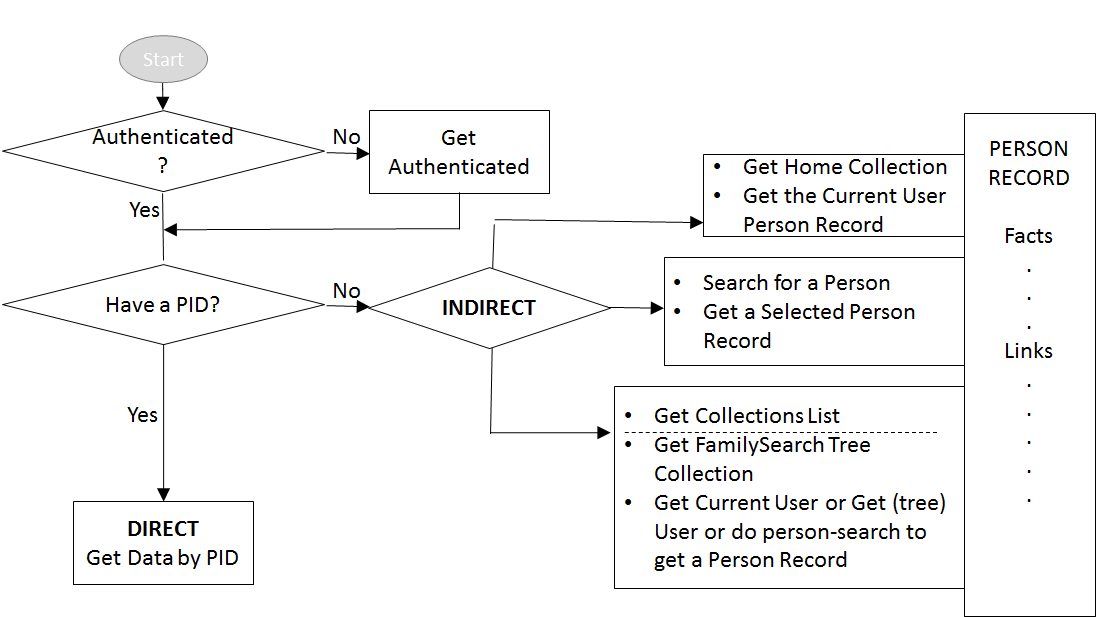
\includegraphics[width=\linewidth]{05/08_dataAccessPaths}
        \centering
        \caption{Sistemes d'accés a les dades de l'arbre familiar}\label{fig:dataAcessPath}
    \end{figure}


    \subsection{L'accés directe a les dades}

        \paragraph{}
        L'accés directe a les dades es pot realitzar si es coneix l'identificador del recurs que vol ser consultat.

        Per exemple, si es coneix el PID de la persona a consultar, es pot codificar des de les aplicacions el diferent conjunt d'URIs per manipular els recursos i evitar així la necessitat de passar pel sistema. D'aquesta forma, es pot doncs accedir a la informació de la persona, memòries, discussions, fills, pares, parelles, avantpassats i descendència; sempre i quan, es conegui tota la informació necessària per codificar les diferents URIs d'accés.

        Un exemple d'ús, podria ser per exemple, donat un identificador de persona conegut, accedir directament a les seves memòries mitjançant la codificació de la URI i evitar, així, haver de passar per l'arbre familiar.


    \subsection{L'accés indirecte a les dades}

        \paragraph{}
        A pesar que poder accedir directament a les dades, pot semblar un procés ideal, el més normal és que ens trobem en la situació de necessitar realitzar un accés indirecte a les dades. En altres paraules, accedir en primera instància als recursos del sistema i obtenir així els diferents enllaços que ens condueixin cap a les operacions desitjades.

        Per descobrir l’URI del recurs exacte que vol ser consultat, existeixen principalment tres opcions diferents:

        \begin{itemize}
            \item Llegir la col·lecció Arrel, que representa la col·lecció que conté totes les dades de FamilySearch i seguir-la per tal d'obtenir l'usuari identificat. Un cop es disposa de la persona relacionada a l'usuari, es pot accedir a qualsevol altre recurs mitjançant els enllaços hypermedia de la resposta i simular, de forma dinàmica, el mateix que podríem haver realitzat mitjançant l'accés directe.
            \item Llegir la llista de col·leccions disponibles per tal d'accedir a l'arbre familiar o accedir a ell de forma directa. Un cop es disposa de l'arbre familiar es pot llegir l'usuari actual o la persona de l'usuari i d'aquí procedir com es desitgi. Una alternativa és accedir mitjançant els enllaços o plantilles URL, als recursos generals de Memòries, Discussions, Relacions, etcètera i consultar la informació general d'aquests recursos mitjançant els seus identificadors retornats.
            \item La tercera opció, i probablement la més comuna, passa per la realització d'una cerca contra la base de dades de FamilySearch per tal d'obtenir una Persona o Localització. Un cop s'obté el resultat de la cerca, es pot navegar a qualsevol de les peces d'informació relacionades als recursos consultats, mitjançant les URI i enllaços hypermedia de les respostes.
        \end{itemize}

        El procés descrit en el tercer punt de les opcions de cerca indirecta, serà el més comú de cara a accedir a la informació, ja que les altres opcions no permeten gaire filtratge de les dades, a menys que coneguem la col·lecció específica sobre la qual volem realitzar una investigació genealògica o només vulguem consultar la informació de l'arbre familiar, de l'usuari identificat.

        Com hem comentat doncs, són quatre les principals opcions d'entrada que permeten obtenir persones concretes de l'arbre de forma indirecta i començar a navegar, des de la resposta d'aquestes, per les dades genealògiques.

        En els següents apartats,  s'explicarà en més detall com poden ser configurades cada una d'aquestes operacions.


    \subsection{Lectura de l'usuari identificat}

        \paragraph{}
        Aquesta operació pot ser realitzada de forma directe, accedint a la URI:

        \begin{displayquote}
            \emph{/platform/users/current}
        \end{displayquote}

        La crida retorna la informació específica del recurs Usuari descrita en els apartats anteriors d'aquesta memòria. Des d'aquest, es pot accedir a la persona de l'arbre familiar que representa a l'usuari i des d’aquesta, a qualsevol altre peça d'informació genealògica relacionada amb la persona.


    \subsection{Lectura de la persona relacionada a l'usuari identificat}

        Aquesta operació és realitzable a través de la URI:

        \begin{displayquote}
            \emph{/platform/tree/current-person}
        \end{displayquote}

        L'operació en qüestió retorna el recurs Persona de l'usuari identificat, amb tota la informació descrita en els apartats anteriors de la memòria. Des d'aquest, es pot navegar a qualsevol altre recurs o dada genealògica relacionada.

        Aquesta forma d'accés representa un pas menys que l’exposada en l’apartat anterior, si sabem d'entrada que volem accedir a l'arbre familiar. En cas que també volguéssim alguna dada del recurs Usuari, caldria entrar per la funcionalitat descrita en l'apartat anterior.


    \subsection{Cerca de Persones a l'arbre familiar}

        \paragraph{}
        L'operació cerca de persones, a l'arbre familiar, és sense cap dubte la més interessant de totes les funcionalitats que ofereix l'API.

        Aquesta operació es realitza mitjançant una petició a la URI /platform/tree/search, que a més a més, pot ser configurada i personalitzada mitjançant la inclusió de diferents paràmetres.

        Un cop finalitzada la petició, aquesta retorna el conjunt de persones de l'arbre familiar, que compleixen amb les condicions imposades en la cerca. L'usuari, pot començar a navegar per la resposta, accedint a aquelles persones que li resultin de més interès i a tots els altres recursos disponibles relacionats amb aquestes.

        Es pot entendre la funcionalitat de cerca a l'arbre familiar, com una porta a totes les dades emmagatzemades per FamilySearch.

        La cerca pot ser controlada mitjançant tres paràmetres principals, un dels quals, accepta molts paràmetres secundaris. Els paràmetres principals són descrits a la taula~\ref{res:searchPersonMain}.

        \begin{center}
                 \csvreader[
                    separator=comma,
                    before table=\sffamily\small,
                    respect tilde=true,
                    respect leftbrace=true,
                    respect rightbrace=true,
                    longtable={p{2cm-2\tabcolsep}p{12cm-2\tabcolsep}},
                    table head={\caption{Variables principals per la cerca de persones}\label{res:searchPersonMain}\\\toprule%
                        \headentry{m{2cm-2\tabcolsep}}{Variable}
                        & \headentry{m{12cm-2\tabcolsep}}{Descripció}\\\midrule},
                    late after line=\\\midrule,
                    late after last line=\\\bottomrule,
                 ]
                 {./tables/05/10_search/searchPersonMain.csv}
                 {var=\var,desc=\desc}
                 {\var&\desc}
         \end{center}

         El paràmetre \emph{q}, descrit en la taula~\ref{res:searchPersonMain}, accepta com a paràmetres vàlids els camps exposats a la taula~\ref{res:searchPersonSec}. L'etiqueta \{relation\}, dels camps d'aquesta taula,  pot ser reemplaçada per qualsevol dels següents valors: father, mother, spouse (pare, mare, parella).

         \begin{center}
                  \csvreader[
                     separator=comma,
                     before table=\sffamily\small,
                     respect tilde=true,
                     respect leftbrace=true,
                     respect rightbrace=true,
                     longtable={p{4cm-2\tabcolsep}p{10cm-2\tabcolsep}},
                     table head={\caption{Paràmetres acceptats per la variable q}\label{res:searchPersonSec}\\\toprule%
                         \headentry{m{4cm-2\tabcolsep}}{Variable}
                         & \headentry{m{10cm-2\tabcolsep}}{Descripció}\\\midrule},
                     late after line=\\\midrule,
                     late after last line=\\\bottomrule,
                  ]
                  {./tables/05/10_search/searchPersonSec.csv}
                  {param=\param,desc=\desc}
                  {\param&\desc}
          \end{center}


          \subsubsection{Cerca de persones duplicades}

          \paragraph{}
          Una característica interessant de les respostes en la cerca de persones és que per cada persona de la resposta, es pot accedir al conjunt de persones de l'arbre familiar, que amb alta probabilitat, poden representar a la mateixa persona consultada. En altres paraules, persones que podrien tractar-se de possibles duplicats.

          Aquesta funcionalitat de cerca de persones duplicades, també es troba accessible mitjançant una URI pròpia, si es coneix l'identificador personal de la persona sobre la qual es vol buscar els possibles duplicats.


    \subsection{Cerca de localitzacions}

        \paragraph{}
        La cerca de localitzacions és la segona opció de cerca massiva que permet l'API de FamilySearch.

        Aquesta operació cobra especial interès quan es necessita consultar informació extra sobre una localització, més enallà de la informació bàsica relacionada a certs recursos de l'arbre familiar, o es vol obtenir informació sobre totes les localitzacions  que compleixen amb certs criteris. Per exemple, totes les localitzacions dins d'una jurisdicció específica.

        Així doncs, la cerca de localitzacions permet relacionar o interpretar, el nom d'una localització, mitjançant una descripció estandarditzada a la URI:

        \begin{displayquote}
            \emph{/platform/places/search}
        \end{displayquote}

        De la mateixa forma que en la cerca de persones, la cerca de localitzacions pot ser configurada mitjançant tres paràmetres principals, on un d'aquests accepta diversos paràmetres secundaris. Els paràmetres principals són descrits a la taula~\ref{res:searchLocMain}.

        \begin{center}
                 \csvreader[
                    separator=comma,
                    before table=\sffamily\small,
                    respect tilde=true,
                    respect leftbrace=true,
                    respect rightbrace=true,
                    longtable={p{2cm-2\tabcolsep}p{12cm-2\tabcolsep}},
                    table head={\caption{Variables principals per la cerca de localitzacions}\label{res:searchLocMain}\\\toprule%
                        \headentry{m{2cm-2\tabcolsep}}{Variable}
                        & \headentry{m{12cm-2\tabcolsep}}{Descripció}\\\midrule},
                    late after line=\\\midrule,
                    late after last line=\\\bottomrule,
                 ]
                 {./tables/05/10_search/searchLocMain.csv}
                 {var=\var,desc=\desc}
                 {\var&\desc}
         \end{center}

         En aquesta operació, el paràmetre \emph{q}, accepta com a vàlids el conjunt de paràmetres especificats a la taula~\ref{res:searchLocSec}.

         \begin{center}
                  \csvreader[
                     separator=comma,
                     before table=\sffamily\small,
                     respect tilde=true,
                     respect leftbrace=true,
                     respect rightbrace=true,
                     longtable={p{2cm-2\tabcolsep}p{10cm-2\tabcolsep}},
                     table head={\caption{Paràmetres acceptats per la variable q}\label{res:searchLocSec}\\\toprule%
                         \headentry{m{2cm-2\tabcolsep}}{Variable}
                         & \headentry{m{10cm-2\tabcolsep}}{Descripció}\\\midrule},
                     late after line=\\\midrule,
                     late after last line=\\\bottomrule,
                  ]
                  {./tables/05/10_search/searchLocSec.csv}
                  {param=\param,desc=\desc}
                  {\param&\desc}
          \end{center}

